\documentclass{article}

\usepackage{graphicx}
\usepackage{hyperref}

\title{\textbf{jettl} \\ An Interface-Composition based LabVIEW Asynchronous Actor Framework}
\author{Nathan Davis}
\date{\today}

\begin{document}

\maketitle

\maketitle

\section{Introduction}
\label{sec:introduction}

Strictly interface composition based asynchronous actor oriented design pattern for LabVIEW Applications.
jettl also has the newer banners for vis. Easy adoption for the new age of LV developers.
State pattern with decorators.
It is interface composition, so stick with the same rule set for naming methods

\section{Philosophy}
\label{sec:philosophy}

\subsection{Access Scope}
\label{subsec:access-scope}

Only public and private.
Interfaces, classes, and methods have text in the icon/banner that are black for public and red for private.

\subsection{Errors}
\label{subsec:errors}

No error goes unrecognized

\section{Class Hierarchy}
\label{sec:class-hierarchy}

\begin{figure}[ht]
    \centering
    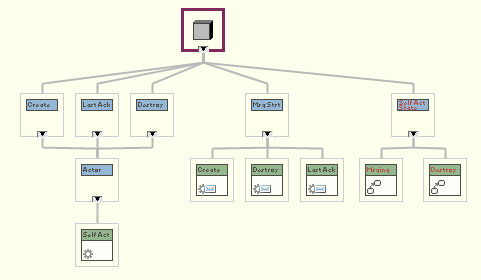
\includegraphics[width=0.8\textwidth]{figures/class-hierarchy}
    \caption{jettl Class Hierarchy.}
    \label{fig:jettl-class-hierarchy}
\end{figure}

Fig~\ref{fig:jettl-class-hierarchy} shows the class hierarchy of jettl.
In particular, there exist design patterns such as the Strategy Pattern, State Pattern, and Decorator Pattern.

\section{Actors}
\label{sec:actors}

\subsection{Actor Benefits}
\label{subsec:actor-benefits}

Actors do not create their own references OR destroy their own references.
They conform to the tree like hierarchy of creation where Caller owns nesteds reference i.e. Caller received Nesteds Last Ack, safe to release their reference.
Actors are queue based.

\section{LabVIEW Interfaces}
\label{sec:labview-interfaces}

The default implementation idea works so only as there is only one method implementation across all interfaces.

For example, \\
class implements interface 1 and interface 2 \\
interface 1: method \\
interface 2: method \\
This cannot exist unless the class overrides the method.
Otherwise, at runtime, LabVIEW does not know to execute interface 1: method or interface 2: method.

\subsection{Descendants Must Override}
\label{subsec:descendants-must-override}

Interface methods: check the 'descendants must override' checkbox and see which errors pop up.
Attempt to fix them, and if you can't, then justify the reasoning.

For example, in the Self Actor State.lvclass, the DD methods are not required to be overridden.
This is because the Self Actor State.lvclass has default functionality in the interface methods.
Maybe this is bad practice, but it is a design choice showing only the methods that are required to be overridden with different functionality.

Another example, the DD methods in the Dev Actor.lvclass are not required to be overridden.
This is because the methods here are all decorator methods that are not required to be overridden.
Using the Actor.lvclass methods are sufficient for the Dev Actor.lvclass.
These will be found in the palette.

\section{Future Scope}
\label{sec:future-scope}

Creating an actor is NOT connected to the actor that creates it.
Rather, this actor exists on its own in the “liquid” message transport.
The overall “application” has access to the actor's reference (unique message address)

\subsection{Pub-Sub Messaging}
\label{subsec:pub-sub-messaging}

\begin{figure}[ht]
    \centering
    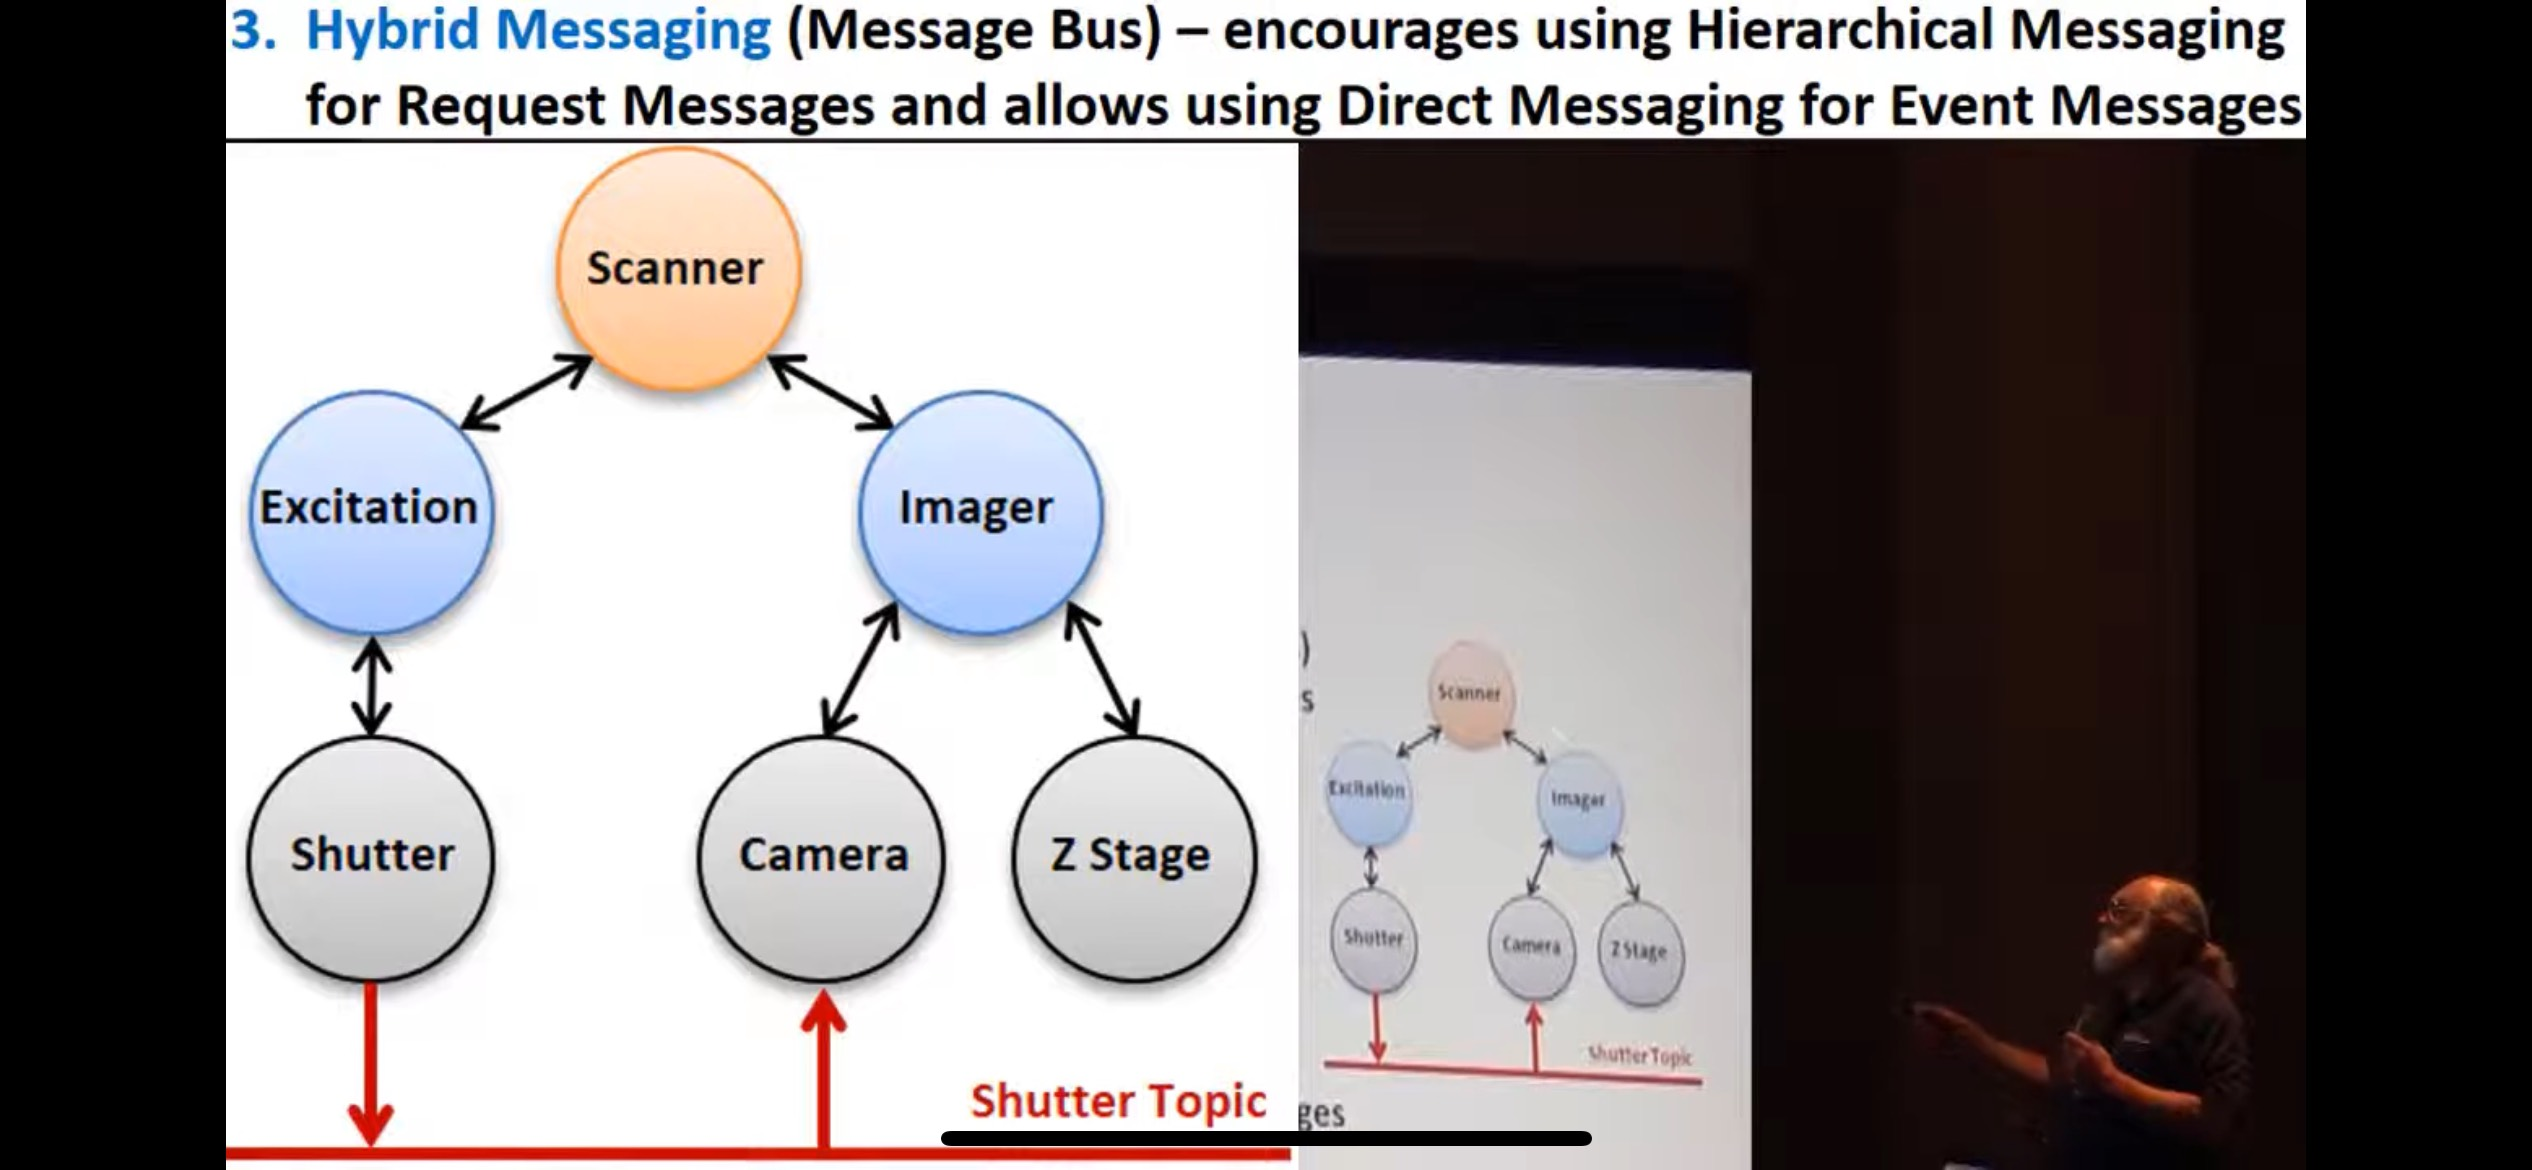
\includegraphics[width=0.8\textwidth]{figures/labview_dmitry_message _transport}
    \caption{LabVIEW Actor Framework Message Transport.}
    \label{fig:message-transport}
\end{figure}

As shown in Fig~\ref{fig:message-transport}, it is as though the actors are just objects that “float” in this “liquid” messaging transport.
So that way you can perform this pub-sub messaging.
The objects are linked together by “who launches who”.

Same as with the pub-sub pattern, everything is a publisher-subscriber.
It's just that most relationships are just one way.
Same with Git, the philosophy is that all branches are created equal

\section{Debugging}
\label{sec:debugging}

\subsection{Displaying Method Execution}
\label{subsec:displaying-method-execution}

What a log for which methods are executed, instead of the dialog popups

Two project conditional blocks:
\begin{enumerate}
    \item Occurs in all methods
    \item Occurs only in message specific methods
\end{enumerate}

These conditionals occur in Self Actor.lvclass.
If either conditional is true, debug panel that displays the names of actors (columns), along with timestamps (rows) of when methods (data) are executed.
Think discrete time water fall display.

\subsection{Debug General LabVIEW}
\label{subsec:debug-general-labview}

General way to see which methods are being executed in the system?
Used to see which actors are presently running / which methods are used?

\section{Git}
\label{sec:git}

This might be of interest for submodules in git for LabVIEW.
Find here: \href{https://www.youtube.com/watch?v=iv7WwDgyb0U}{Git Submodules: An Alternative Approach to Code Reuse - Greg Payne - GDevCon2}.

In the repos, use the tag to have different "stable" versions of the repo such as v0.1.1 or v3.8.3
This allows others to easily look at the different versions of the repo without much thought.
This could also help with submodules that are referenced in other repos.
Check this video near the end for reference: \href{https://www.youtube.com/watch?v=tRZGeaHPoaw&list=PLvDxiIkwuMQs0Uu6AIhTGqXahndMmfUyx&index=19}{Git and GitHub Tutorial for Beginners}

\section{Naming Conventions}
\label{sec:naming-conventions}

\begin{figure}[ht]
    \centering
    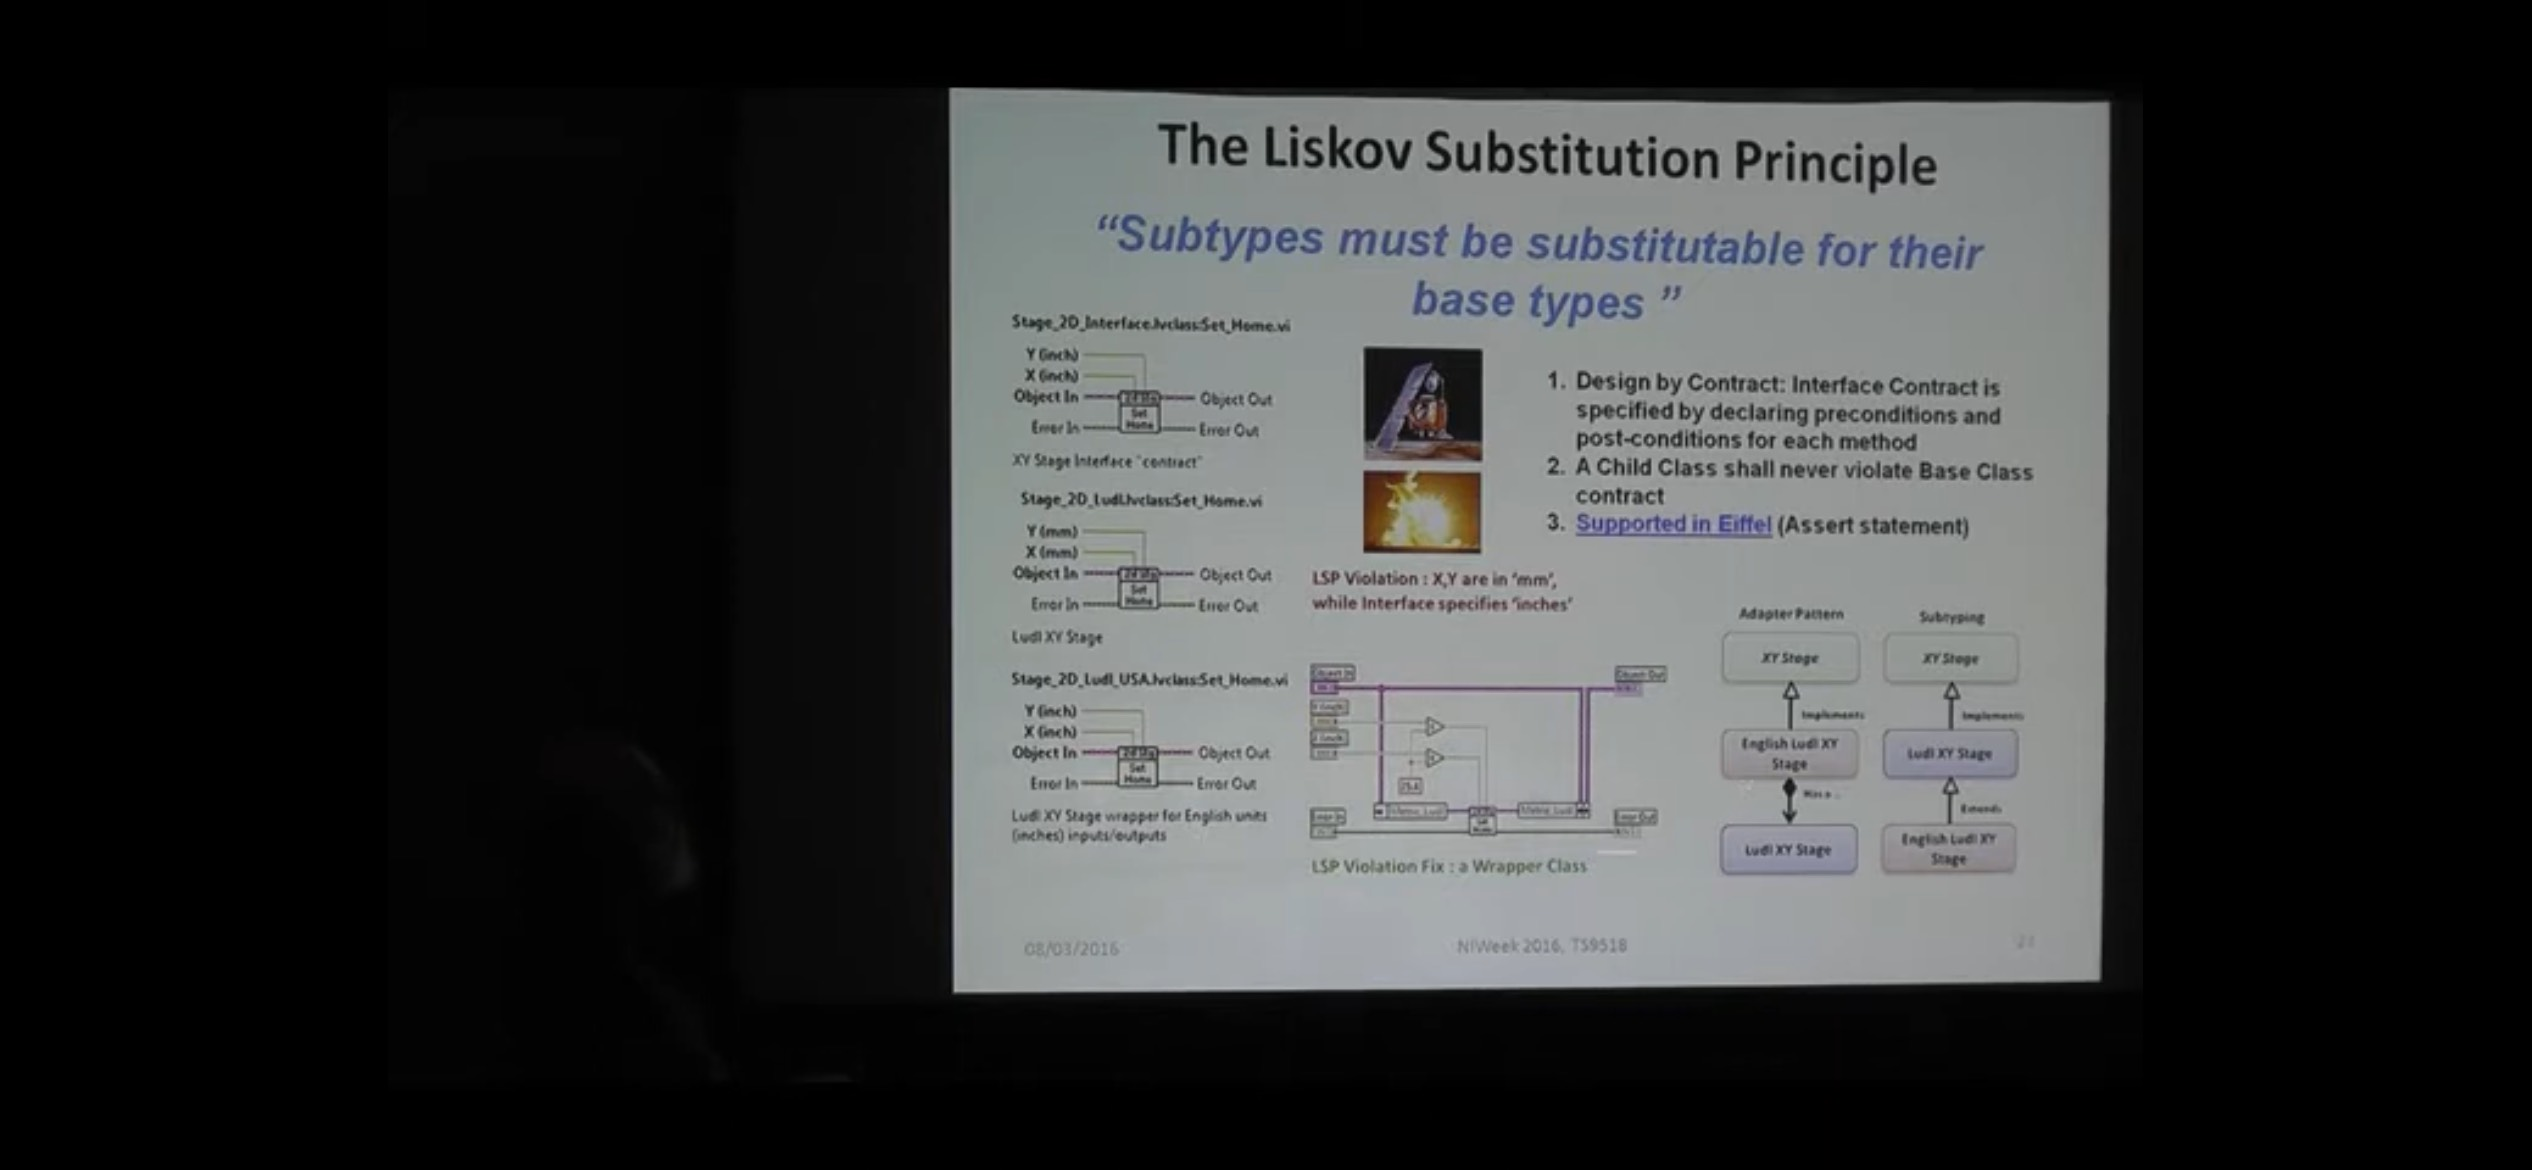
\includegraphics[width=0.8\textwidth]{figures/dmitry_liskov_sub_principle}
    \caption{This image shows the naming convention for LabVIEW classes and methods.}
    \label{fig:dmitry-liskov-sub-principle}
\end{figure}

Noting that Fig~\ref{fig:dmitry-liskov-sub-principle} shows the naming convention for LabVIEW classes and methods.
\begin{itemize}
    \item{Library-Name.lvlib}
    \item{Interface-Name.lvclass}
    \item{Class-Name.lvclass (control is capital by default!)}
    \item{method-Name.vi}
    \item{control-Name.ctl (this control, which is not tied to a class is lowercase!)}
\end{itemize}

\noindent Note: Avoid underscores and spaces.

\section{Design Patterns}
\label{sec:design-patterns}

\subsection{State Pattern}
\label{subsec:state-pattern}

\noindent Context:

\quad Method.vi (just a wrapper for Method.vi “State”).\footnote{Best Practice: use this Method.vi in other methods, rather than the Method.vi “State” itself}

\noindent State.lvclass (interface):

\quad Concrete State.lvclass

\quad Method.vi “State”

\subsection{Memento Pattern}
\label{subsec:memento-pattern}

When saving the state of an actor, the Memento Pattern is used.
Instead of sending the entire actor state in Actor Last Ack Msg, there should be another dedicated message that sends the actors state to the calling actor.
This has not been done, but it is a good idea to implement this in the future.

Memento, actors shouldn't know about each other, so if the state of a nested is to be saved, then there is a separate message for this since last ack shouldn't know about this.
Rather, this specialty message couples with last ack if the developer wants this functionality.

\section{External Packages}
\label{sec:external-packages}

\href{https://www.vipm.io/package/illuminatedg_lib_ig_oopanel/}{IG OOPanel}

\section{Helper Loops}
\label{sec:helper-loops}

\subsection{Helper Loop Best Practices}
\label{subsec:helper-loop-best-practices}

References cannot change after they are created.

\subsection{Helper Loop Benefits}
\label{subsec:helper-loop-benefits}

They are orphan processes since they create and release their own references.
They are not tied to the actor that launches them.
Furthermore, they are not tied to the lifetime of the actor that launches them.
Helper Loops are event based.

\subsection{Panels}
\label{subsec:panels}

Actor helpers, not helper actors.
Helper Loop → Async Actor Helper.
These are helper loops that are created async which help an actor with its task.
This is to declutter the actor by offloading certain tasks such as panel display or subprocesses that do not require an additional actor to be created.

Modular UI.
Since the UIs and its references' dependency is NOT dependent on the actor, we can unit test the UIs.

\subsection{UI Events}
\label{subsec:ui-events}

Indicators: Instead of generating an event, bundle in the reference of the indicator and have a property node (write)in the subVI.

The same can be said for the control, which has a right click menu, that bundles in the reference for the control and creates a subVI that writes the value to the front panel.
Or creates a signal, something that automatically puts the control in the event loop and bundles in the reference for the control to the subVI.
Create control which does the same as the indicators but added the reference of the control to the private data.

In prelaunch, have a subVI that internally has the creation of the user events.
Script to create the subVI first.

Interface with DD methods:
No need for template to replace the placeholder methods with new ones, just have DD methods as “placeholders” which change their implementation depending on the class that's on the wire

\begin{figure}[ht]
    \centering
    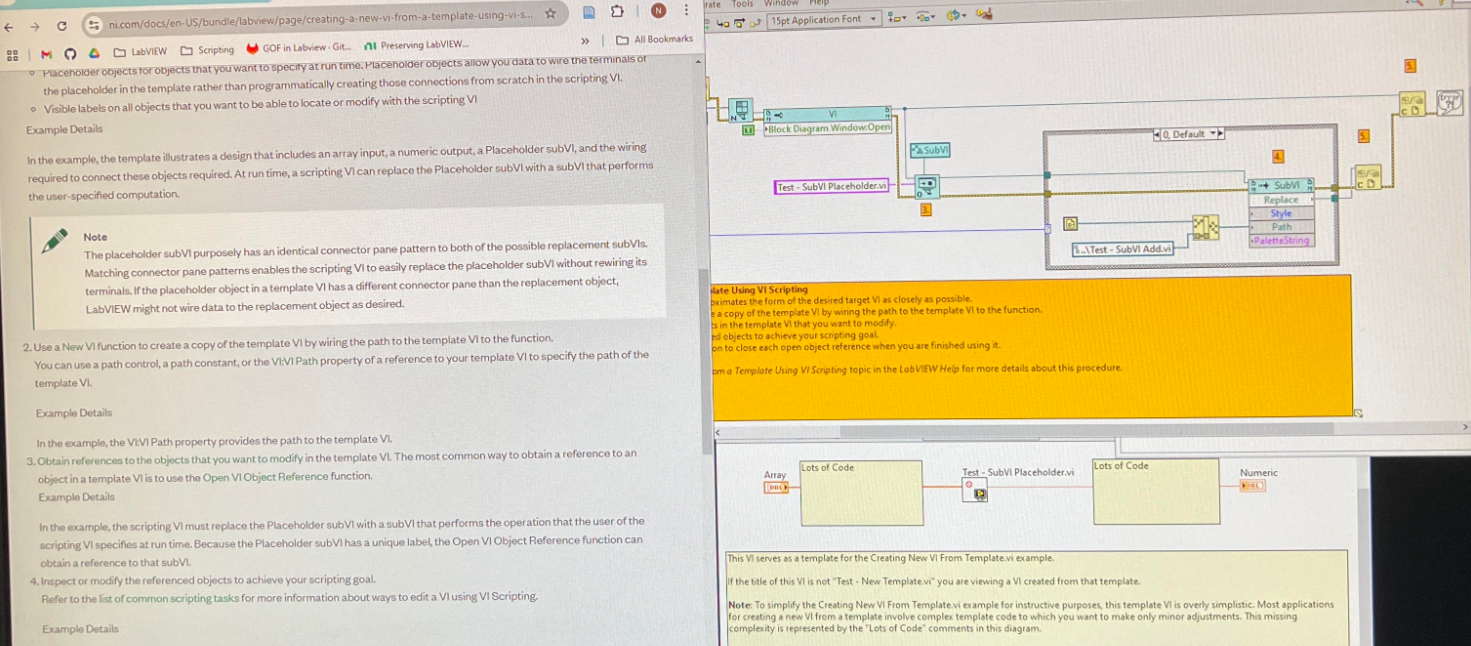
\includegraphics[width=0.8\textwidth]{figures/justACS_ui_events}
    \caption{This image shows the UI events in LabVIEW.}
    \label{fig:justacs-ui-events}
\end{figure}

Split the events as controls and indicators as shown in Fig~\ref{fig:justacs-ui-events}.

\subsection{Right Click creates library with interface}

Method in actor: \\
Creates library containing interface and method along with message class with Send and Do methods

\section{Messaging}
\label{sec:messaging}

All messages come from an interface and follow ISP where one message belongs to one interface.
If there is a naming issue, that is a good thing.
It means in the dependencies, you should be packaging modules so you don't run into naming issues.


All messages are interface messages.
Note, they do not need to be implemented.

Actor messages error on generation of message.
Error when creating a message and wiring in the interface object as an input, the message scripting doesn't know how to differentiate the class input and the parameter input.

\subsection{Error Msg}
\label{subsec:error-msg}

\begin{figure}
    \centering
    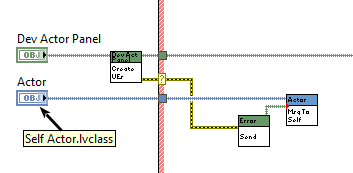
\includegraphics[width=0.8\textwidth]{figures/Need_for_error_msg}
    \caption{Error message in jettl. This is a custom error message that occurs when an error occurs asynchronously.}
    \label{fig:error-msg}
\end{figure}

\section{Scripting}
\label{sec:scripting}

Go through and replace all the Opens and Traverse with the hidden gem.

User groups for the scripting (quick drop, right click, etc.).


\section{TODO}
\label{sec:todo}

Rename Error to Actor Error.

Check execution for all methods.

Have the interface checkbox for DD methods not required for override doesn't necessarily break subtype rules!

In the DD methods, because they are not required to be overridden, have functionality within them that calls the Self Actor method (some kind of checking mechanism?).

Actor interface methods (all implemented with default functionality) to have the *new* (Actor Interface) Read Actor DD method that reads from the Dev Actor the Self Actor class and performs that interface function, then bundles back in with the Setup method.

Do this for all for the default behavior.

Note this is breaking the contract for interface DD methods not needing to be overridden.

Instead of the Setup method, create a new Actor Write method which ONLY Writes to the Actor. This can also be put inside the Setup method as a first step, the setup code follows after

State Enter Core and State Exit Core are NOT check marked.
That way the developer does not need to override, just to have no functionality anyway.
Read State and Write State do because they'll have functionality.

\section{Miscellaneous}
\label{sec:miscellaneous}

\subsection{MEF (Managed Extensibility Framework)}
\label{subsec:mef}

\href{https://www.youtube.com/watch?v=rrtz7sKCg2A}{LabVIEW Interfaces for Satellite Calibration - SLM and McBee}: 44:50

\section{Errors}
\label{sec:errors}

In frameworks, errors are fundamental to the program's operation. They are not just incidental issues but rather integral to the design and flow of the application.
jettl has an error object in the private data of the jettl object. At the end of the method, the error object is unbundled and checked for errors before teardown.

Error philosophy: Errors occur ONLY from unexpected events.
For example, the error case in Msg.vi: in the case structure, a custom error saying that a message could not be executed occurs when 'message name' occurs for 'actor name'. This is unexpected behavior since this SHOULD be known at edit time. This is a legit error.

'That was handled, or I wouldn't have been called' - SLM (\href{https://www.youtube.com/watch?v=00TZxeyt8_A}{The Errors of our Ways | Stephen Loftus-Mercer GDevCon N.A. 2021: 52:08})

\begin{figure}[ht]
    \centering
    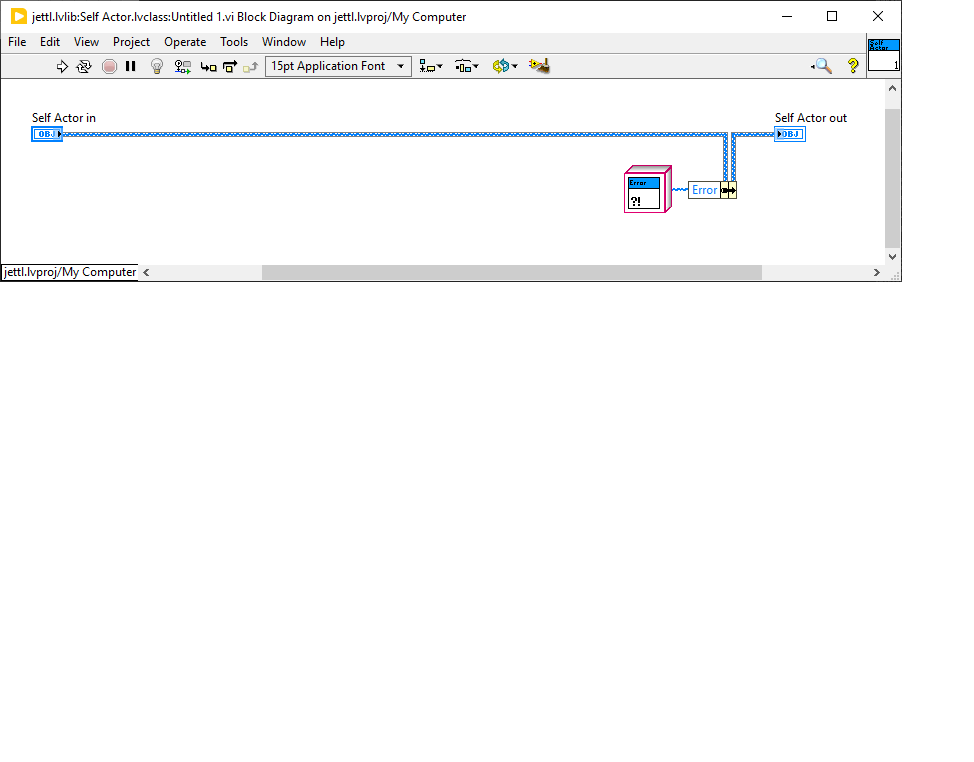
\includegraphics[width=0.8\textwidth]{figures/method-template}
    \caption{Method template. This has no error terminals, and the error cluster is handled internally. This is a different approach to error handling in LabVIEW methods.}
    \label{fig:method-template}
\end{figure}
% have the actual method template here, from the example. These are scripted and autogenerated when one creates an actor.

Wouldn't this make the API more beautiful and easy to understand? Having just the object wire come out of the method, and ONLY the object wire coming out of the method?
I suppose, adopting the OO paradigm.
Instead of having the error cluster inside the objects class data.
Instead, it's a dedicated “error cluster” shared for every single object in use.
Encourages data flow since unbundling of errors will always occur.
It's a step in the right direction having no “error input” for methods.
Now it's time to get rid of the error out.
It's almost like branching an objects wire, in a way. There should only be one thing coming out of a method.

\section{Orderly Shutdown}
\label{sec:orderly-shutdown}

Boolean flag for orderly shutdown i.e.'destroy nested actors before destroying self'

\section{Example}
\label{sec:example}

\subsection{Dev Actor}
\label{subsec:dev-actor}

No decorators used since they're trivial and only used once.

\end{document}
